% Copyright (c) 2011 Martin Ueding <dev@martin-ueding.de>

\part{ROOT}

\chapter{Übung 10}

\begin{figure}[h]
\begin{center}
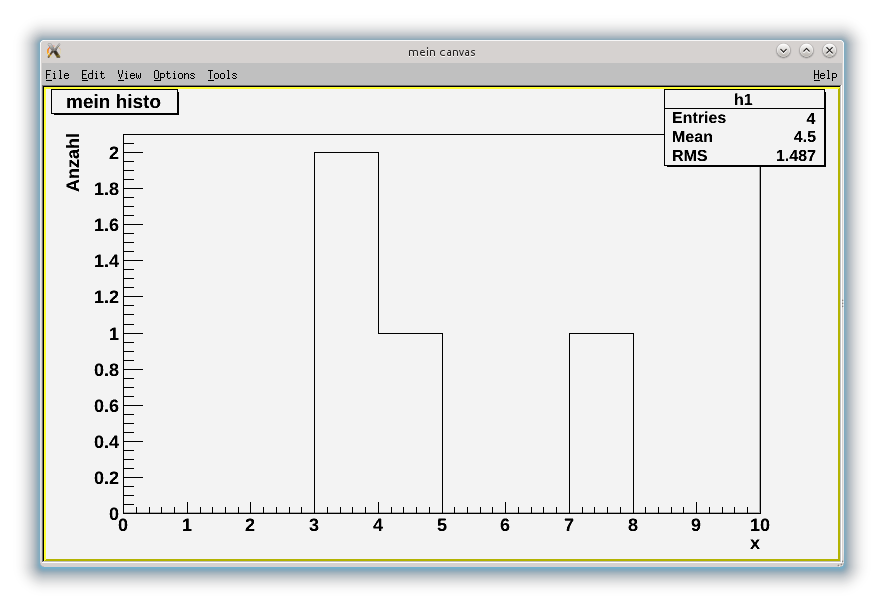
\includegraphics[width=10cm]{Uebung_10/default.png}
\caption{Standardplot}
\end{center}
\end{figure}



\begin{figure}[h]
\begin{center}
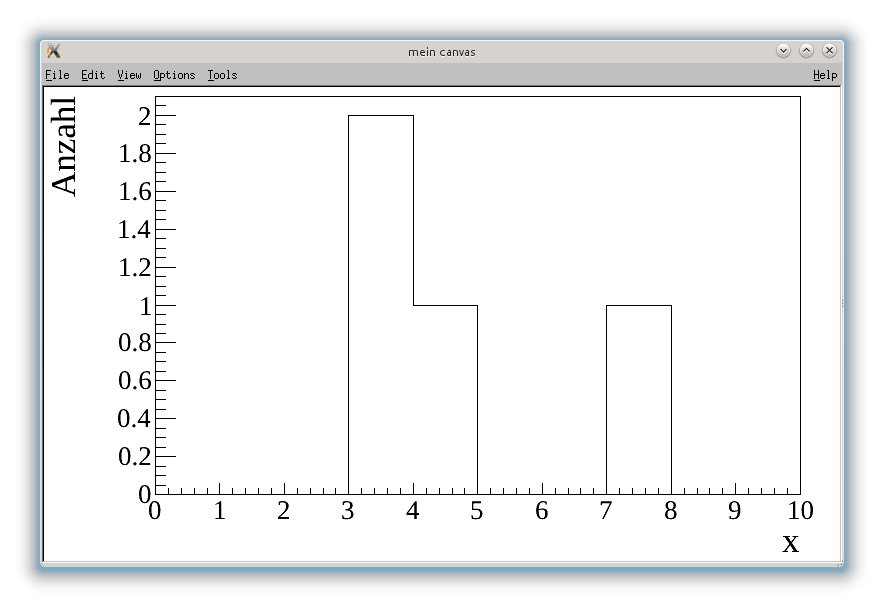
\includegraphics[width=10cm]{Uebung_10/babar.png}
\caption{BABAR Plot}
\end{center}
\end{figure}

Man kann mit \texttt{c1->SetLogx(1)} eine logarithmische Achse aktivieren und mit \texttt{c1->SetLogx(0)} wieder zurück zur linearen Achse wechseln.

\section{Berichtsaufgabe}

\code[c++]{Uebung_10/bericht.C}{Code für Plot}{code:root1}

\begin{table}[h]
\begin{center}
\begin{tabular}{rclcl}
Chi2 & = & 48.4851 &  \\ 
NDf & = & 17 &  \\ 
p0 & = & -0.153455 & $\pm$ & 0.0434887 \\ 
p1 & = & 2.04459 & $\pm$ & 0.00707916 \\ 
\end{tabular} 
\caption{Parameter des Fits}
\label{table:fit}
\end{center}
\end{table}


\begin{figure}[h]
\begin{center}
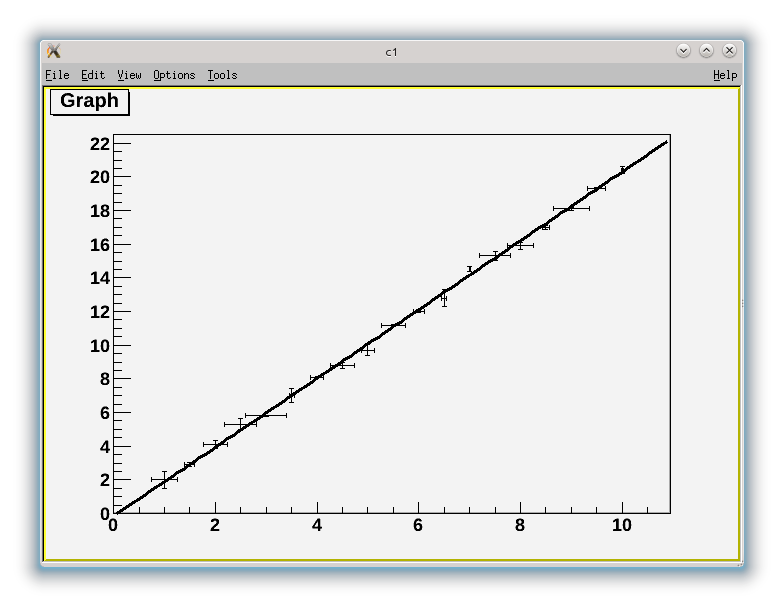
\includegraphics[width=10cm]{Uebung_10/fit.png}
\caption{Messwerte mit linearem Fit}
\end{center}
\end{figure}